% !LW recipe = lualatex-draft -> biber -> lualatex*2
%╔════════════════════════════╗
%║	  Szablon dostosował	  ║
%║	        Kotlarski         ║
%║		  06.10.2024		  ║
%╚════════════════════════════╝
\documentclass[12pt,oneside,a4paper,openany]{article}

    % ------------------------------------------------------------------------
% PAKIETY
% ------------------------------------------------------------------------

%różne pakiety matematyczne, warto przejrzeć dokumentację, muszą być powyżej ustawień językowych.
\usepackage{mathrsfs}   %Różne symbole matematyczne opisane w katalogu ~\doc\latex\comprehensive. Zamienia \mathcal{L} ze zwykłego L na L-transformatę.
\usepackage{eucal}      %Różne symbole matematyczne.
\usepackage{amssymb}    %Różne symbole matematyczne.
\usepackage{amsmath}    %Dodatkowe funkcje matematyczne, np. polecenie \dfac{}{} skladajace ulamek w trybie wystawionym (porównaj $\dfrac{1}{2}$, a $\frac{1}{2}$).

%język polski i klawiatura
\usepackage[polish]{babel}
\usepackage{csquotes}
%\usepackage{qtimes} % czcionka Times new Roman
\usepackage{polski}

\usepackage{ifluatex}

\ifluatex
  %czcionka
  \usepackage{fontspec} % pozwalający na użycie czcionek systemowych
  \setmainfont{lato} % czcionka Calibri (problem na Linuxie)

  %obsługa pdf'a
  \usepackage[luatex,usenames,dvipsnames]{color}      %Obsługa kolorów. Opcje usenames i dvipsnames wprowadzają dodatkowe nazwy kolorow.
	\usepackage[luatex,pagebackref=false,draft=false,pdfpagelabels=false,colorlinks=true,urlcolor=black,linkcolor=black,filecolor=black,citecolor=black,pdfstartview=FitH,pdfstartpage=1,pdfpagemode=UseOutlines,bookmarks=true,bookmarksopen=true,bookmarksopenlevel=2,bookmarksnumbered=true,pdfauthor={imie nazwisko},pdftitle={Dokumentacja Projektowa},pdfsubject={},pdfkeywords={transient recovery voltage trv},unicode=true]{hyperref}   %Opcja pagebackref=true dotyczy bibliografii: pokazuje w spisie literatury numery stron, na których odwołano się do danej pozycji.
\else
  \usepackage[pdftex,usenames,dvipsnames]{color}      %Obsługa kolorów. Opcje usenames i dvipsnames wprowadzają dodatkowe nazwy kolorow.
\usepackage[pdftex,pagebackref=false,draft=false,pdfpagelabels=false,colorlinks=true,urlcolor=black,linkcolor=black,filecolor=black,citecolor=black,pdfstartview=FitH,pdfstartpage=1,pdfpagemode=UseOutlines,bookmarks=true,bookmarksopen=true,bookmarksopenlevel=2,bookmarksnumbered=true,pdfauthor={imie nazwisko},pdftitle={Dokumentacja Projektowa},pdfsubject={},pdfkeywords={transient recovery voltage trv},unicode=true]{hyperref}  %Opcja pagebackref=true dotyczy bibliografii: pokazuje w spisie literatury numery stron, na których odwołano się do danej pozycji.
\fi

\usepackage{lastpage} %! do numerowania stron w formacie (x z y) Alternatywnie można użyć \label{LastPage} na ostatniej stronie w dokumrnt.tex 

%bibliografia
%\usepackage[numbers,sort&compress]{natbib}  %Porządkuje zawartość odnośników do literatury, np. [2-4,6]. Musi być pod pdf'em, a styl bibliogfafii musi mieć nazwę z dodatkiem 'nat', np. \bibliographystyle{unsrtnat} (w kolejności cytowania).
\usepackage[
backend=biber,
style=numeric,
sorting=none
]{biblatex}
\addbibresource{bibliografia.bib}
\usepackage{hypernat}                       %Potrzebna pakietowi natbib do wspolpracy z pakietem hyperref (wazna kolejnosc: 1. hyperref, 2. natbib, 3. hypernat).

%grafika i geometria strony
\usepackage{extsizes}           %Dostepne inne rozmiary czcionek, np. 14 w poleceniu: \documentclass[14pt]{article}.
\usepackage[final]{graphicx}
\usepackage{circuitikz}
\ctikzset{logic ports=american}
\usepackage{subcaption}
\usepackage[a4paper,left=2cm,right=2cm,top=2cm,bottom=2cm,headheight=24pt]{geometry}

%strona tytułowa
\usepackage{strona_tytulowa}

%inne
\usepackage[hide]{todo}                     %Wprowadza polecenie \todo{treść}. Opcje pakietu: hide/show. Polecenie \todos ma byc na koncu dokumentu, wszystkie \todo{} po \todos sa ignorowane.
\usepackage[basic,physics]{circ}            %Wprowadza środowisko circuit do rysowania obwodów elektrycznych. Musi byc poniżej pakietow językowych.
\usepackage[sf,bf,outermarks]{titlesec}     %Troszczy się o wygląd tytułów rozdziałów (section, subsection, ...). sf oznacza czcionkę sans serif (typu arial), bf -- bold. U mnie: oddzielna linia dla naglowku paragraph. Patrz tez: tocloft -- lepiej robi format spisu tresci.
\usepackage{tocloft}                        %Troszczy się o format spisu trsci.
\usepackage{expdlist}    %Zmienia definicję środowiska description, daje większe możliwości wpływu na wygląd listy.
\usepackage{flafter}     %Wprowadza parametr [tb] do polecenia \suppressfloats[t] (polecenie to powoduje nie umieszczanie rysunkow, tabel itp. na stronach, na ktorych jest to polecenie (np. moze byc to stroma z tytulem rozdzialu, ktory chcemy zeby byl u samej gory, a nie np. pod rysunkiem)).
\usepackage{array}       %Ładniej drukuje tabelki (np. daje wiecej miejsca w komorkach -- nie są tak ścieśnione, jak bez tego pakietu).
\usepackage{listings}    %Listingi programow.
\usepackage[format=hang,labelsep=period,labelfont={bf,small},textfont=small]{caption}   %Formatuje podpisy pod rysunkami i tabelami. Parametr 'hang' powoduje wcięcie kolejnych linii podpisu na szerokosc nazwy podpisu, np. 'Rysunek 1.'.
\usepackage{appendix}    %Troszczy się o załączniki.
\usepackage{floatflt}    %Troszczy się o oblewanie rysunkow tekstem.
\usepackage{here}        %Wprowadza dodtkowy parametr umiejscowienia rysunków, tabel, itp.: H (duże). Umiejscawia obiekty ruchome dokladnie tam gdzie są w kodzie źródłowym dokumentu.
\usepackage{makeidx}     %Troszczy się o indeks (skorowidz).

%nieużywane, ale potencjalnie przydatne
\usepackage{sectsty}           %Formatuje nagłówki, np. żeby były kolorowe -- polecenie: \allsectionsfont{\color{Blue}}.
%\usepackage{version}           %Wersje dokumentu.

%============
\usepackage{longtable}			%tabelka
\usepackage{tabularx}
\usepackage{booktabs}			%linie \toprule, \midrule, \bottomrule w tabelach
\usepackage{siunitx}			%jednostki SI: \SI{2}{\minute}, \SI{90}{\degree}
%============

%============
% Ustawienia listingów do kodu
%============

\usepackage{listings}
\usepackage{xcolor}

\definecolor{codegreen}{rgb}{0,0.6,0}
\definecolor{codegray}{rgb}{0.5,0.5,0.5}
\definecolor{codepurple}{rgb}{0.58,0,0.82}
\definecolor{backcolour}{rgb}{0.95,0.95,0.92}

% Definicja stylu "mystyle"
\lstdefinestyle{mystyle}{
	backgroundcolor=\color{backcolour},   
	commentstyle=\color{codegreen},
	keywordstyle=\color{blue},	%magenta
	numberstyle=\tiny\color{codegray},
	stringstyle=\color{codepurple},
	basicstyle=\ttfamily\footnotesize,
	breakatwhitespace=false,         
	breaklines=true,                 
	captionpos=b,                    
	keepspaces=true,                 
	numbers=left,                    
	numbersep=5pt,                  
	showspaces=false,                
	showstringspaces=false,
	showtabs=false,                  
	tabsize=2,
	literate=
	  {á}{{\'a}}1 {é}{{\'e}}1 {í}{{\'i}}1 {ó}{{\'o}}1 {ú}{{\'u}}1
	{Á}{{\'A}}1 {É}{{\'E}}1 {Í}{{\'I}}1 {Ó}{{\'O}}1 {Ú}{{\'U}}1
	{à}{{\`a}}1 {è}{{\`e}}1 {ì}{{\`i}}1 {ò}{{\`o}}1 {ù}{{\`u}}1
	{À}{{\`A}}1 {È}{{\`E}}1 {Ì}{{\`I}}1 {Ò}{{\`O}}1 {Ù}{{\`U}}1
	{ä}{{\"a}}1 {ë}{{\"e}}1 {ï}{{\"i}}1 {ö}{{\"o}}1 {ü}{{\"u}}1
	{Ä}{{\"A}}1 {Ë}{{\"E}}1 {Ï}{{\"I}}1 {Ö}{{\"O}}1 {Ü}{{\"U}}1
	{â}{{\^a}}1 {ê}{{\^e}}1 {î}{{\^i}}1 {ô}{{\^o}}1 {û}{{\^u}}1
	{Â}{{\^A}}1 {Ê}{{\^E}}1 {Î}{{\^I}}1 {Ô}{{\^O}}1 {Û}{{\^U}}1
	{ã}{{\~a}}1 {ẽ}{{\~e}}1 {ĩ}{{\~i}}1 {õ}{{\~o}}1 {ũ}{{\~u}}1
	{Ã}{{\~A}}1 {Ẽ}{{\~E}}1 {Ĩ}{{\~I}}1 {Õ}{{\~O}}1 {Ũ}{{\~U}}1
	{œ}{{\oe}}1 {Œ}{{\OE}}1 {æ}{{\ae}}1 {Æ}{{\AE}}1 {ß}{{\ss}}1
	{ű}{{\H{u}}}1 {Ű}{{\H{U}}}1 {ő}{{\H{o}}}1 {Ő}{{\H{O}}}1
	{ç}{{\c c}}1 {Ç}{{\c C}}1 {ø}{{\o}}1 {Ø}{{\O}}1 {å}{{\r a}}1 {Å}{{\r A}}1
	{€}{{\euro}}1 {£}{{\pounds}}1 {«}{{\guillemotleft}}1
	{»}{{\guillemotright}}1 {ñ}{{\~n}}1 {Ñ}{{\~N}}1 {¿}{{?`}}1 {¡}{{!`}}1
	{ą}{{\k{a}}}1 {ć}{{\'{c}}}1 {ę}{{\k{e}}}1 {ł}{{\l}}1 {ń}{{\'n}}1
	{ó}{{\'o}}1 {ś}{{\'s}}1 {ź}{{\'z}}1 {ż}{{\.{z}}}1
	{Ą}{{\k{A}}}1 {Ć}{{\'{C}}}1 {Ę}{{\k{E}}}1 {Ł}{{\L}}1 {Ń}{{\'N}}1
	{Ó}{{\'O}}1 {Ś}{{\'S}}1 {Ź}{{\'Z}}1 {Ż}{{\.{Z}}}1
	}

	% Styl dla Electron + Vue + TypeScript (frontend)
\lstdefinestyle{frontend}{
    basicstyle=\ttfamily\footnotesize,
    keywordstyle=\color{teal!70!black}\bfseries,
    commentstyle=\color{gray!60}\itshape,
    stringstyle=\color{green!60!black},
    numbers=left,
    numberstyle=\ttfamily\tiny\color{gray}\raisebox{0.5ex},
    stepnumber=1,
    numbersep=5pt,
    breaklines=true,
    frame=single,
    backgroundcolor=\color{teal!5},
    showspaces=false,
    showstringspaces=false,
    showtabs=false,
    tabsize=2,
    captionpos=b,
    linewidth=\linewidth,
    xleftmargin=20pt,
    xrightmargin=5pt,
    framexleftmargin=15pt,
    framexrightmargin=5pt,
    rulecolor=\color{teal!30},
    literate={ą}{{\k{a}}}1
             {ć}{{\'c}}1
             {ę}{{\k{e}}}1
             {ł}{{\l{}}}1
             {ń}{{\'n}}1
             {ó}{{\'o}}1
             {ś}{{\'s}}1
             {ź}{{\'z}}1
             {ż}{{\.z}}1
             {Ą}{{\k{A}}}1
             {Ć}{{\'C}}1
             {Ę}{{\k{E}}}1
             {Ł}{{\L{}}}1
             {Ń}{{\'N}}1
             {Ó}{{\'O}}1
             {Ś}{{\'S}}1
             {Ź}{{\'Z}}1
             {Ż}{{\.Z}}1
             {{<}}{{$<$}}1
             {{>}}{{$>$}}1
             {{~}}{{${\sim}$}}1
             {{_}}{{\_}}1
             {{^}}{{${\hat}$}}1
             {{°}}{{$^{\circ}$}}1,
    keywords={abstract, as, async, await, boolean, break, case, catch, class, 
      const, continue, declare, default, delete, do, else, enum, export, 
      extends, false, finally, for, from, function, get, if, implements, import, in, 
      instanceof, interface, keyof, let, module, namespace, never, new, null, 
      number, object, private, protected, public, readonly, require, return, 
      set, static, string, super, switch, symbol, this, throw, true, try, type, typeof, 
      undefined, unknown, var, void, while, with, yield,
      // Electron specific
      app, BrowserWindow, ipcMain, ipcRenderer, dialog, Menu, Tray, 
      shell, clipboard, nativeImage, screen, globalShortcut, powerMonitor,
      // Vue specific
      ref, reactive, computed, watch, onMounted, onUnmounted, onBeforeMount,
      defineComponent, nextTick, provide, inject, readonly, shallowRef, toRefs,
      // TypeScript specific
      type, interface, enum, namespace, module, declare, implements},
    emph={app, BrowserWindow, ipcMain, ref, reactive, computed, onMounted, defineComponent},
    emphstyle=\color{teal!80!black},
    lineskip=2pt,
    aboveskip=10pt,
    belowskip=10pt,
    numberblanklines=false,
    morecomment=[l]{//},
    morecomment=[s]{/*}{*/},
    morestring=[b]`,
    morestring=[b]'
}

% Styl dla Hono + TypeScript (backend)
\lstdefinestyle{backend}{
    basicstyle=\ttfamily\footnotesize,
    keywordstyle=\color{red!60!black}\bfseries,
    commentstyle=\color{gray!60}\itshape,
    stringstyle=\color{green!60!black},
    numbers=left,
    numberstyle=\ttfamily\tiny\color{gray}\raisebox{0.5ex},
    stepnumber=1,
    numbersep=5pt,
    breaklines=true,
    frame=single,
    backgroundcolor=\color{red!5},
    showspaces=false,
    showstringspaces=false,
    showtabs=false,
    tabsize=2,
    captionpos=b,
    linewidth=\linewidth,
    xleftmargin=20pt,
    xrightmargin=5pt,
    framexleftmargin=15pt,
    framexrightmargin=5pt,
    rulecolor=\color{red!30},
    literate={ą}{{\k{a}}}1
             {ć}{{\'c}}1
             {ę}{{\k{e}}}1
             {ł}{{\l{}}}1
             {ń}{{\'n}}1
             {ó}{{\'o}}1
             {ś}{{\'s}}1
             {ź}{{\'z}}1
             {ż}{{\.z}}1
             {Ą}{{\k{A}}}1
             {Ć}{{\'C}}1
             {Ę}{{\k{E}}}1
             {Ł}{{\L{}}}1
             {Ń}{{\'N}}1
             {Ó}{{\'O}}1
             {Ś}{{\'S}}1
             {Ź}{{\'Z}}1
             {Ż}{{\.Z}}1
             {{<}}{{$<$}}1
             {{>}}{{$>$}}1
             {{~}}{{${\sim}$}}1
             {{_}}{{\_}}1
             {{^}}{{${\hat}$}}1
             {{°}}{{$^{\circ}$}}1,
    keywords={abstract, as, async, await, boolean, break, case, catch, class, 
      const, continue, declare, default, delete, do, else, enum, export, 
      extends, false, finally, for, from, function, get, if, implements, import, in, 
      instanceof, interface, keyof, let, module, namespace, never, new, null, 
      number, object, private, protected, public, readonly, require, return, 
      set, static, string, super, switch, symbol, this, throw, true, try, type, typeof, 
      undefined, unknown, var, void, while, with, yield,
      // Hono specific
      Hono, Context, Next, Middleware, serve, serveStatic, cors, logger, 
      jwt, basicAuth, etag, compress, prettyJSON, secureHeaders, timeout,
      get, post, put, delete, patch, options, head, route, use, all, on,
      // TypeScript specific
      type, interface, namespace, module, declare, implements, Pick, Omit, Partial, Required},
    emph={Hono, Context, Next, get, post, put, delete, serve, cors, logger, jwt},
    emphstyle=\color{red!80!black},
    lineskip=2pt,
    aboveskip=10pt,
    belowskip=10pt,
    numberblanklines=false,
    morecomment=[l]{//},
    morecomment=[s]{/*}{*/},
    morestring=[b]`,
    morestring=[b]'
}

% Styl dla C++ + TypeScript (dodatki - binding/native modules)
\lstdefinestyle{cpp}{
    basicstyle=\ttfamily\footnotesize,
    keywordstyle=\color{brown!70!black}\bfseries,
    commentstyle=\color{gray!60}\itshape,
    stringstyle=\color{green!60!black},
    numbers=left,
    numberstyle=\ttfamily\tiny\color{gray},
    stepnumber=1,
    numbersep=5pt,
    breaklines=true,
    frame=single,
    backgroundcolor=\color{brown!10},
    showspaces=false,
    showstringspaces=false,
    showtabs=false,
    tabsize=2,
    captionpos=b,
    linewidth=\linewidth,
    xleftmargin=20pt,
    xrightmargin=5pt,
    framexleftmargin=15pt,
    framexrightmargin=5pt,
    rulecolor=\color{brown!30},
    literate={ą}{{ą}}1
             {ć}{{ć}}1
             {ę}{{ę}}1
             {ł}{{ł}}1
             {ń}{{ń}}1
             {ó}{{ó}}1
             {ś}{{ś}}1
             {ź}{{ź}}1
             {ż}{{ż}}1
             {Ą}{{Ą}}1
             {Ć}{{Ć}}1
             {Ę}{{Ę}}1
             {Ł}{{Ł}}1
             {Ń}{{Ń}}1
             {Ó}{{Ó}}1
             {Ś}{{Ś}}1
             {Ź}{{Ź}}1
             {Ż}{{Ż}}1,
    keywords={auto, bool, break, case, catch, char, class, const, constexpr, continue, 
      default, delete, do, double, else, enum, explicit, export, extern, false, 
      float, for, friend, goto, if, inline, int, long, namespace, new, noexcept, 
      nullptr, operator, private, protected, public, register, reinterpret_cast, 
      return, short, signed, sizeof, static, static_assert, static_cast, struct, 
      switch, template, this, throw, true, try, typedef, typeid, typename, union, 
      unsigned, using, virtual, void, volatile, while,
      type, interface, module, declare, export, import, const, let, function,
      napi_value, napi_env, napi_callback, napi_deferred, NAPI_CALL, 
      napi_create_object, napi_set_named_property, napi_get_named_property,
      optional, vector, uint8_t, string_view, nullopt, size_t, nullptr, mmap,
      PROT_READ, MAP_SHARED},
    emph={napi_value, napi_env, class, constexpr, template, type, interface, 
          NAPI_CALL, optional, vector, uint8_t},
    emphstyle=\color{brown!80!black},
    lineskip=2pt,
    aboveskip=10pt,
    belowskip=10pt,
    numberblanklines=false,
    morecomment=[l]{//},
    morecomment=[s]{/*}{*/},
    morestring=[b]",
    morestring=[b]',
    extendedchars=true,
    inputencoding=utf8,
    deletekeywords={nullptr},
    keepspaces=true,
    columns=flexible
}
	

\lstset{style=mystyle} % Deklaracja aktywnego stylu
%===========
\usepackage{rotating}    %Obracanie tekstu i rysunków (np. diagramy poziome)
%============

% dodatkowe do emotek LuaLaTeX

\ifluatex
  \usepackage{fontspec}
\fi
\usepackage{pifont}   % for \ding symbols
\usepackage{xcolor}   % for yellow color

%PAGINA GÓRNA I DOLNA
\usepackage{fancyhdr}          %Dodaje naglowki jakie się chce.
\pagestyle{fancy}
\fancyhf{}
% numery stron na środku dolnej stopki
\fancyfoot[C]{\footnotesize DOKUMENTACJA LABORATORIUM - SYSTEMY WBUDOWANE\\ 
\normalsize\sffamily  \thepage\ z~\pageref{LastPage}}


%\fancyhead[L]{\small\sffamily \nouppercase{\leftmark}}
\fancyhead[C]{\footnotesize \textit{AKADEMIA NAUK STOSOWANYCH W NOWYM SĄCZU}\\}

\renewcommand{\headrulewidth}{0.4pt}
\renewcommand{\footrulewidth}{0.4pt}

    % ------------------------------------------------------------------------
% USTAWIENIA
% ------------------------------------------------------------------------

% ------------------------------------------------------------------------
%   Kropki po numerach sekcji, podsekcji, itd.
%   Np. 1.2. Tytuł podrozdziału
% ------------------------------------------------------------------------
\makeatletter
    \def\numberline#1{\hb@xt@\@tempdima{#1.\hfil}}                      %kropki w spisie treści
    \renewcommand*\@seccntformat[1]{\csname the#1\endcsname.\enspace}   %kropki w treści dokumentu
\makeatother

% ------------------------------------------------------------------------
%   Numeracja równań, rysunków i tabel
%   Np.: (1.2), gdzie:
%   1 - numer sekcji, 2 - numer równania, rysunku, tabeli
%   Uwaga ogólna: o otoczeniu figure ma być najpierw \caption{}, potem \label{}, inaczej odnośnik nie działa!
% ------------------------------------------------------------------------
\makeatletter
    \@addtoreset{equation}{section} %resetuje licznik po rozpoczęciu nowej sekcji
    \renewcommand{\theequation}{{\thesection}.\@arabic\c@equation} %dodaje kropki

    \@addtoreset{figure}{section}
    \renewcommand{\thefigure}{{\thesection}.\@arabic\c@figure}

    \@addtoreset{table}{section}
    \renewcommand{\thetable}{{\thesection}.\@arabic\c@table}
\makeatother

% ------------------------------------------------------------------------
% Tablica
% ------------------------------------------------------------------------
\newenvironment{tabela}[3]
{
    \begin{table}[!htb]
    \centering
    \caption[#1]{#2}
    \vskip 9pt
    #3
}{
    \end{table}
}

% ------------------------------------------------------------------------
% Dostosowanie wyglądu pozycji listy \todos, np. zamiast 'p.' jest 'str.'
% ------------------------------------------------------------------------
\renewcommand{\todoitem}[2]{%
    \item \label{todo:\thetodo}%
    \ifx#1\todomark%
        \else\textbf{#1 }%
    \fi%
    (str.~\pageref{todopage:\thetodo})\ #2}
\renewcommand{\todoname}{Do zrobienia...}
\renewcommand{\todomark}{~uzupełnić}

% ------------------------------------------------------------------------
% Definicje
% ------------------------------------------------------------------------
\def\nonumsection#1{%
    \section*{#1}%
    \addcontentsline{toc}{section}{#1}%
    }
\def\nonumsubsection#1{%
    \subsection*{#1}%
    \addcontentsline{toc}{subsection}{#1}%
    }
\reversemarginpar %umieszcza notki po lewej stronie, czyli tam gdzie jest więcej miejsca
\def\notka#1{%
    \marginpar{\footnotesize{#1}}%
    }
\def\mathcal#1{%
    \mathscr{#1}%
    }
\newcommand{\atp}{ATP/EMTP} % Inaczej: \def\atp{ATP/EMTP}

% ------------------------------------------------------------------------
% Inne
% ------------------------------------------------------------------------
\frenchspacing                      
\hyphenation{ATP-EMTP}             %dzielenie wyrazu w danym miejscu
\setlength{\parskip}{3pt}           %odstęp pomiędzy akapitami
\linespread{1.3}                    %odstęp pomiędzy liniami (interlinia)
\setcounter{tocdepth}{4}            %uwzględnianie w spisie treści czterech poziomów sekcji
\setcounter{secnumdepth}{4}         %numerowanie do czwartego poziomu sekcji 
\titleformat{\paragraph}[hang]      %wygląd nagłówków
{\normalfont\sffamily\bfseries}{\theparagraph}{1em}{}

%komenda do łatwiejszego wstawiania zdjęć
% Parametr #1 (opcjonalny): Szerokość zdjęcia (domyślnie \textwidth)
% Parametr #2: Nazwa pliku z rozszerzeniem (np. rys/nazwa-rysunku.png)
% Parametr #3: Opis rysunku wyświetlany pod rysunkiem
% Parametr #4: Identyfikator rysunku (do oznaczania zdjęć w tekście)
\newcommand*{\fg}[4][\textwidth]{
    \begin{figure}[!htb]
        \begin{center}
            \includegraphics[width=#1]{#2}
            \caption{#3}
            \label{rys:#4}
        \end{center}
    \end{figure}
}

%komenda do oznaczania elementów w tekście
% Parametr #1: Typ elementu (rys, lst)
% Parametr #2: Identyfikator elementu
\newcommand*{\Oznacz}[2]{
\ref{#1:#2} (s. \pageref{#1:#2})
}

%komenda do oznaczania zdjęć w tekście
% Parametr #1 (opcjonalny): Nazwa typu elementu (domyślnie Rysunek)
% Parametr #2: Identyfikator rysunku
\newcommand*{\OznaczZdjecie}[2][Rysunek]{
#1 \Oznacz{rys}{#2}
}

%komenda do oznaczania kodu w tekście
% Parametr #1: Identyfikator kodu
\newcommand*{\OznaczKod}[1]{
\Oznacz{lst}{#1}
}

%komenda do wstawiania listingów kodu
% Parametr #1: Opis listingu wyświetlany pod listingiem
% Parametr #2: Identyfikator listingu
% Parametr #3: Ścieżka do pliku z kodem
\newcommand*{\ListingFile}[3]{
    \lstinputlisting[caption=#1, label={lst:#2}, language=C++]{#3}
}

\newcommand{\Tick}{\textcolor{green}{\ding{52}}\quad
}
\newcommand{\Cross}{\textcolor{red}{\ding{56}}\quad
}
\newcommand{\Triangle}{\textcolor{orange}{$\blacktriangle$}\quad
}

    %polecenia zdefiniowane w pakiecie strona_tytulowa.sty
    \title{"Implementacja własnego przykładu \\ drabinkowego układu kombinacyjnego"}		%...Wpisać nazwę projektu...
    \author{Arkadiusz Ryczek}
    \authorI{}
    \authorII{}		%jeśli są dwie osoby w projekcie to zostawiamy:    \authorII{}
    \authorIII{}			%jeśli są trzy osoby w projekcie to zostawiamy:    \authorIII{}
		
	\uczelnia{AKADEMIA NAUK STOSOWANYCH \\W NOWYM SĄCZU}
    \instytut{Wydział Nauk Inżynieryjnych}
    \kierunek{Katedra Informatyki}
    \praca{SPRAWOZDANIE Z LABORATORIUM}
    \przedmiot{Systemy wbudowane}
    \prowadzacy{dr inż. Ihor Pazdriy}
    \rok{2026}


%definicja składni mikrotik
\usepackage{fancyvrb}
\DefineVerbatimEnvironment{MT}{Verbatim}%
{commandchars=\+\[\],fontsize=\small,formatcom=\color{red},frame=lines,baselinestretch=1,} 
\let\mt\verb 
%zakonczenie definicji składni mikrotik

\usepackage{fancyhdr}    %biblioteka do nagłówka i stopki

			
\begin{document}
   
    \renewcommand{\figurename}{Rys.}    %musi byc pod \begin{document}, bo w~tym miejscu pakiet 'babel' narzuca swoje ustawienia
    \renewcommand{\tablename}{Tab.}     %j.w.
    \thispagestyle{empty}               %na tej stronie: brak numeru
    \stronatytulowa                     %strona tytułowa tworzona przez pakiet strona_tytulowa.tex
 
 \pagestyle{fancy}

    \newpage

    %formatowanie spisu treści i~nagłówków
    \renewcommand{\cftbeforesecskip}{8pt}
    \renewcommand{\cftsecafterpnum}{\vskip 8pt}
    \renewcommand{\cftparskip}{3pt}
    \renewcommand{\cfttoctitlefont}{\Large\bfseries\sffamily}
    \renewcommand{\cftsecfont}{\bfseries\sffamily}
    \renewcommand{\cftsubsecfont}{\sffamily}
    \renewcommand{\cftsubsubsecfont}{\sffamily}
    \renewcommand{\cftparafont}{\sffamily}
    %koniec formatowania spisu treści i nagłówków
     
    \tableofcontents    %spis treści
    \thispagestyle{fancy}
    \newpage

    
    \newpage

    
%%%%%%%%%%%%%%%%%%% treść główna dokumentu %%%%%%%%%%%%%%%%%%%%%%%%%

   \section{Opis problemu}
\label{sec:problem}

\subsection{Sformułowanie wymagań}
Rozważamy oświetlenie klatki schodowej sterowane z czterech przycisków
monostabilnych $S_1, S_2, S_3, S_4$ (po jednym na każdym piętrze) oraz
z czujnika ruchu oznaczonego dalej jako $M$. Wymagania
funkcjonalne są następujące:

\begin{enumerate}
    \item Światło można \textbf{włączyć} z dowolnego z czterech przycisków
          (gdy jest zgaszone).
    \item Jeżeli światło \textbf{świeci} i zostanie wciśnięty
          \emph{jakikolwiek} przycisk, światło gaśnie.
    \item Jeżeli światło świeci i przez \SI{2}{\minute} czujnik ruchu nie
          wykryje żadnego ruchu, światło gaśnie samoczynnie.
    \item Każde wykrycie ruchu przez czujnik $M$ \textbf{zeruje} odliczanie
          czasu (przedłuża świecenie o kolejne \SI{2}{\minute}).
\end{enumerate}

Punkty 1–2 sprowadzają się do klasycznego zachowania
\emph{przerzutnika typu T} (toggle): każde zbocze narastające sygnału
,,wciśnięto przycisk'' zmienia stan wyjścia $Q$. Punkt 3–4 realizuje
asynchroniczne zerowanie po upływie zadanego czasu bezruchu.

\subsection{Wielkości wejściowe i wyjściowe}
\begin{table}[H]
\centering
\caption{Zestawienie sygnałów układu.}
\begin{tabular}{cll}
\toprule
Symbol & Znaczenie & Typ \\
\midrule
$S_1,\dots,S_4$ & przyciski na piętrach & wejście, chwilowe \\
$M$              & czujnik ruchu     & wejście, poziom \\
$T$              & sygnał przekroczenia \SI{2}{\minute} bezruchu & wewnętrzny \\
$Q$              & stan oświetlenia (1 = świeci) & wyjście \\
\bottomrule
\end{tabular}
\end{table}

\subsection{Założenia projektowe}
\begin{itemize}
    \item Wszystkie przyciski są \emph{monostabilne}, tzn. sygnał jest
          aktywny tylko w trakcie naciśnięcia.
    \item Reakcja na ,,jakikolwiek przycisk'' modelowana jest bramką OR:
          $P = S_1 \lor S_2 \lor S_3 \lor S_4$.
    \item W części cyfrowej zakładamy, że sygnał $T$ jest już wytworzony
          przez timer (np. w mikrokontrolerze). W części 5 pokażemy go
          jako przekaźnik czasowy w schemacie drabinkowym.
    \item Stan wyjścia opisujemy zmienną $Q$; stan następny – $Q_{\text{next}}$.
\end{itemize}
   \section{Model logiczny w postaci bramek}
\label{sec:bramki}

\subsection{Równanie stanu}
Zachowanie przerzutnika T z zerowaniem można opisać zależnością:
\begin{equation}
    Q_{\text{next}} \;=\; \bigl(P \oplus Q\bigr) \,\land\, \lnot T ,
    \label{eq:main}
\end{equation}
gdzie $P = S_1 \lor S_2 \lor S_3 \lor S_4$, a $T$ jest sygnałem
przekroczenia dopuszczalnego czasu bezruchu.

\subsection{Schemat bramkowy}
Rysunek~\ref{fig:bramki} przedstawia realizację równania~\eqref{eq:main}
przy użyciu bramek OR, XOR, AND oraz NOT.

\begin{figure}[H]
\centering
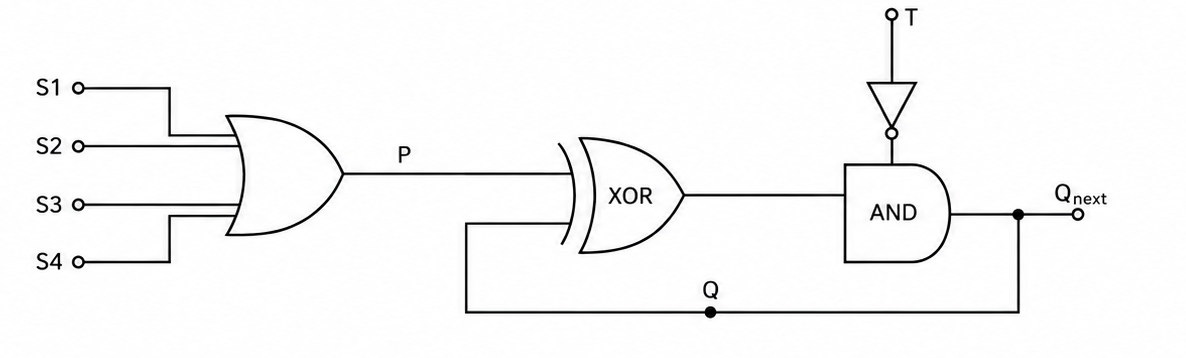
\includegraphics[width=\textwidth]{figures/Blokowy.png}
\caption{Schemat logiczny układu sterowania oświetleniem.}
\label{fig:bramki}
\end{figure}
   \section{Uproszczenie wyrażenia logicznego}
\label{sec:uproszczenie}

Wychodzimy od równania~\eqref{eq:main}:
\begin{align}
    Q_{\text{next}}
    &= (P \oplus Q)\land \lnot T \nonumber\\
    &= (P\lnot Q + \lnot P Q)\,\lnot T \nonumber\\
    &= P\,\lnot Q\,\lnot T \;+\; \lnot P\,Q\,\lnot T .
    \label{eq:sop}
\end{align}

Wyrażenie~\eqref{eq:sop} jest \emph{minimalną} postacią
dysjunkcyjną (SOP). Nie da się jej dalej zredukować bez zmiany
interpretacji fizycznej, ponieważ:
\begin{itemize}
    \item pierwszy składnik $P\bar Q\bar T$ odpowiada sytuacji
          ,,światło zgaszone, przycisk wciśnięty, brak przekroczenia czasu''
          – włączenie światła,
    \item drugi składnik $\bar P Q\bar T$ odpowiada sytuacji
          ,,światło świeci, przycisk wciśnięty, brak przekroczenia czasu''
          – wyłączenie światła.
\end{itemize}

Równoważnie można pozostawić postać z bramką XOR:
\begin{equation}
    Q_{\text{next}} = (P \oplus Q)\,\lnot T,
\end{equation}
która jest korzystniejsza sprzętowo (jedna bramka XOR + jedna AND
zamiast czterech bramek AND, dwóch NOT i jednej OR).

\paragraph{Wniosek.} Realizacja sprzętowa powinna użyć
\textbf{bramki XOR} – pozwala to zaoszczędzić 4 bramki względem
postaci SOP.
   \section{Tabela prawdy}
\label{sec:tabela}

Tabela prawdy dla wyrażenia~\eqref{eq:sop} zawiera $2^3 = 8$ wierszy
(trzy zmienne wejściowe: $Q$, $P$, $T$).

\begin{table}[H]
\centering
\caption{Tabela prawdy układu.}
\label{tab:truth}
\begin{tabular}{ccc|c|l}
\toprule
$Q$ & $P$ & $T$ & $Q_{\text{next}}$ & Interpretacja \\
\midrule
0 & 0 & 0 & 0 & ciemno, brak przycisku, brak przekroczenia czasu \\
0 & 0 & 1 & 0 & ciemno, bez zmian \\
0 & 1 & 0 & 1 & \textbf{włączenie} światła przyciskiem \\
0 & 1 & 1 & 0 & przycisk wciśnięty, ale timeout gasi światło \\
1 & 0 & 0 & 1 & świeci, brak przycisku, brak timeoutu \\
1 & 0 & 1 & 0 & \textbf{automatyczne wyłączenie} po 2 min bezruchu \\
1 & 1 & 0 & 0 & \textbf{wyłączenie} światła przyciskiem \\
1 & 1 & 1 & 0 & timeout wygrywa nad przyciskiem \\
\bottomrule
\end{tabular}
\end{table}

\paragraph{Uwaga projektowa.} W wierszach, w których $T=1$, wyjście
jest zerowane niezależnie od stanu $P$ i $Q$ – jest to zamierzone:
sygnał timeoutu ma najwyższy priorytet (asynchroniczne kasowanie
przerzutnika).
   \section{Schemat drabinkowy (Ladder Diagram)}
\label{sec:drabinka}

\subsection{Postać klasyczna}
Schemat drabinkowy pokazano na rysunku~\ref{fig:ladder}. Zastosowano
następujące oznaczenia:
\begin{itemize}
    \item \texttt{-{}-[\,]-{}-} – styk normalnie otwarty (NO),
    \item \texttt{-{}-[/]-{}-} – styk normalnie zamknięty (NC),
    \item \texttt{-{}-(\,)-{}-} – cewka wyjściowa,
    \item \texttt{TON} – przekaźnik czasowy opóźnionego załączenia
          (\SI{2}{\minute}), zerowany sygnałem $M$.
\end{itemize}

\begin{figure}[H]
\centering
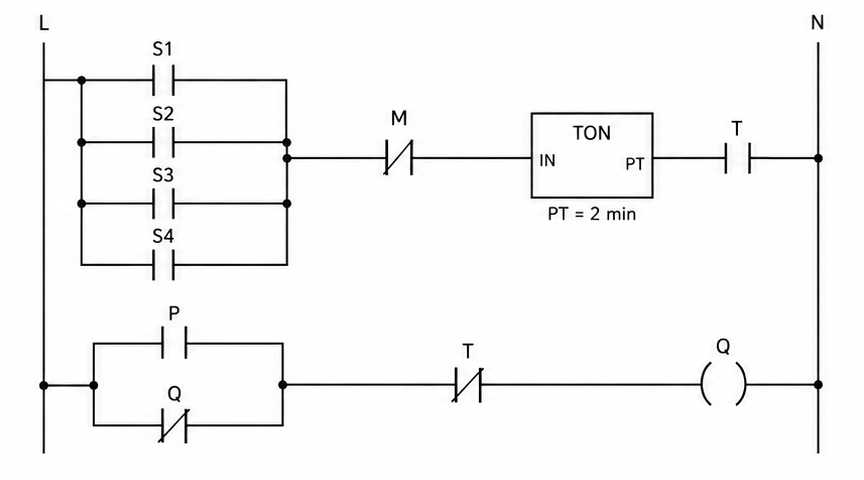
\includegraphics[width=\textwidth]{figures/Drabinkowy.png}
\caption{Schemat drabinkowy sterowania oświetleniem.}
\label{fig:ladder}
\end{figure}

\subsection{Odwzorowanie w programie LOGO!Soft Comfort}
Schemat drabinkowy został odwzorowany w programie LOGO!Soft Comfort na rysunku~\ref{fig:logo_bez_zbocza}. Pierwotnie przyjęto odrobinę błędne założenie, mianowicie nie wzięto pod uwagę faktu, że konieczne będzie użycie dodatkowego bloku wykrywania zbocza (\texttt{AND (edge) - zbocze narastające}). Brak tego bloku spowodował, że wyjście Q1 migotało ze względu na cykliczny charakter pracy sterownika PLC. Podczas przytrzymania przycisku sygnał wejściowy pozostawał w stanie wysokim przez wiele cykli programu, co w połączeniu z logiką XOR powodowało naprzemienne, błyskawiczne załączanie i wyłączanie cewki Q1.

\begin{figure}[H]
\centering
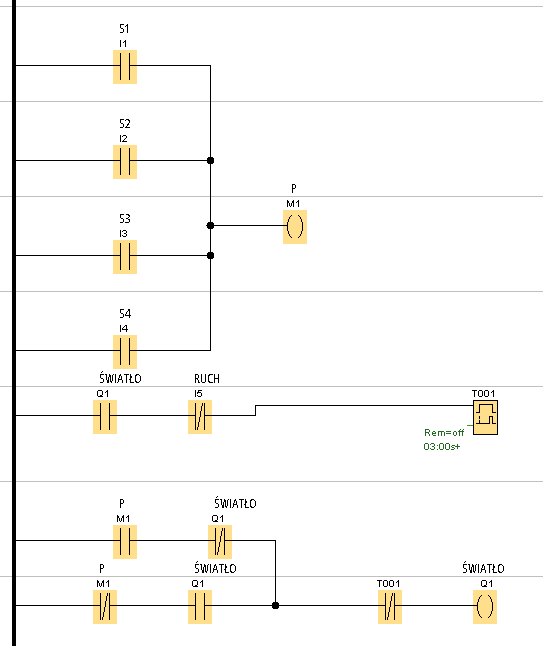
\includegraphics[width=\textwidth]{figures/logo_bez_zbocza.png}
\caption{Schemat drabinkowy odwzorowany w programie LOGO!Soft Comfort.}
\label{fig:logo_bez_zbocza}
\end{figure}

Zastosowanie bloku detekcji zbocza narastającego (SF002) całkowicie rozwiązało ten problem. Zamienia on ciągły sygnał z przycisków na pojedynczy impuls trwający dokładnie jeden cykl programu. Dzięki temu każde fizyczne naciśnięcie przycisku zmienia stan oświetlenia dokładnie raz, co zapewnia stabilną pracę układu. Dodatkowo, prawidłowe wpięcie wyjścia timera (jako styku NC w szeregu z cewką) gwarantuje, że po upływie 2 minut bezruchu światło zostanie asynchronicznie wygaszone, a układ będzie od razu gotowy na przyjęcie kolejnego impulsu z przycisków, bez konieczności resetowania stanów pośrednich. Ostateczna implementacja w pełni odzwierciedla zależność logiczną z równania \eqref{eq:rownanie_stanu} i spełnia wszystkie założenia projektowe.


\begin{figure}[H]
\centering
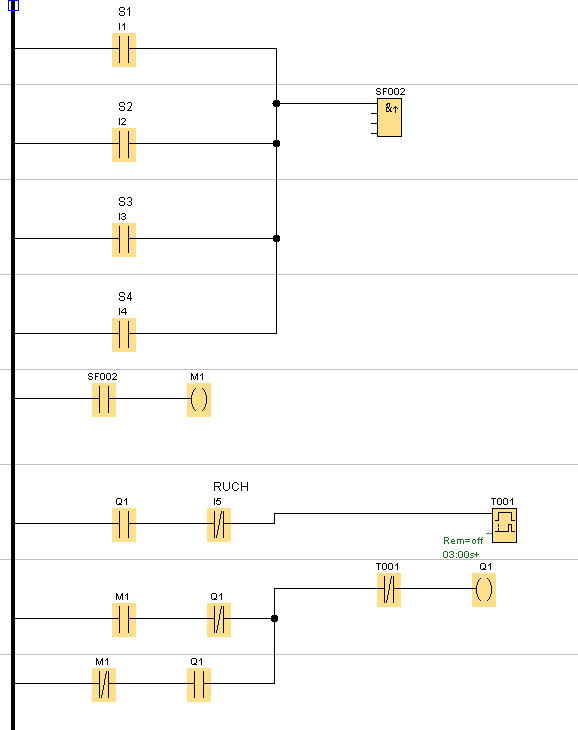
\includegraphics[width=\textwidth]{figures/logo_z_zboczem.png}
\caption{Schemat drabinkowy odwzorowany w programie LOGO!Soft Comfort z użyciem bloku detekcji zbocza narastającego (SF002).}
\label{fig:logo_z_zboczem}
\end{figure}
   
       
%%%%%%%%%%%%%%%%%%% koniec treść główna dokumentu %%%%%%%%%%%%%%%%%%%%%
	\newpage
% \addcontentsline{toc}{section}{Literatura}
% Modified by: zespół projektowy
%Wyświetlanie bibliografii jako "Literatura", w spisie treści wyświetla się podbnie do \section
\printbibliography[heading=bibnumbered, label=Literatura, title=Literatura]

    \newpage
    \hypersetup{linkcolor=black}
    \renewcommand{\cftparskip}{3pt}
    \clearpage
    \renewcommand{\cftloftitlefont}{\Large\bfseries\sffamily}
    \listoffigures
    \addcontentsline{toc}{section}{Spis rysunków}
	\thispagestyle{fancy}
	
    \newpage
    \renewcommand{\cftlottitlefont}{\Large\bfseries\sffamily}
    \def\listtablename{Spis tabel}
    \addcontentsline{toc}{section}{Spis tabel}\listoftables 
	\thispagestyle{fancy}
	
	% \newpage
	% \renewcommand{\cftlottitlefont}{\Large\bfseries\sffamily}
	% \renewcommand\lstlistlistingname{Spis listingów}
	% \addcontentsline{toc}{section}{Spis listingów}\lstlistoflistings 
	% \thispagestyle{fancy}
	


    %lista rzeczy do zrobienia: wypisuje na koñcu dokumentu, patrz: pakiet todo.sty
    \todos
    %koniec listy rzeczy do zrobienia
\end{document}
